
\begin{center}

\includegraphics[width=0.6\textwidth]{content/3/chapter4/images/31.png}\\
Cippi receives the divine touch
\end{center}

Designated initialization is a special case of aggregate initialization. Writing about designated initialization therefore means writing about aggregate initialization.

\subsubsubsection{4.4.1\hspace{0.2cm} Aggregate Initialization}

First: what is an aggregate? Aggregates are arrays and class types. A class type is a class, a struct, or a union.

With C++20, the following condition must hold for class types supporting aggregate initialization:

\begin{itemize}
\item 
No private or protected non-static data members

\item 
No user-declared or inherited constructors

\item 
No virtual, private, or protected base classes

\item 
No virtual member functions
\end{itemize}

The next program exemplifies aggregate initialization.

\noindent
Aggregate initialization
\begin{lstlisting}[style=styleCXX]
// aggregateInitialization.cpp

#include <iostream>

struct Point2D{
	int x;
	int y;
};

class Point3D{
public:
	int x;
	int y;
	int z;
};

int main(){

std::cout << '\n';

	Point2D point2D{1, 2};
	Point3D point3D{1, 2, 3};
	
	std::cout << "point2D: " << point2D.x << " " << point2D.y << '\n';
	std::cout << "point3D: " << point3D.x << " " << point3D.y << " "
							 << point3D.z << '\n';
	
	std::cout << '\n';

}
\end{lstlisting}

Lines 21 and 22 directly initialize the aggregates using curly braces. The sequence of the initializers in the curly braces has to match the declaration order of the members. In the section covering the three-way comparison operator is a more sophisticated example of aggregate initialization.

\begin{center}
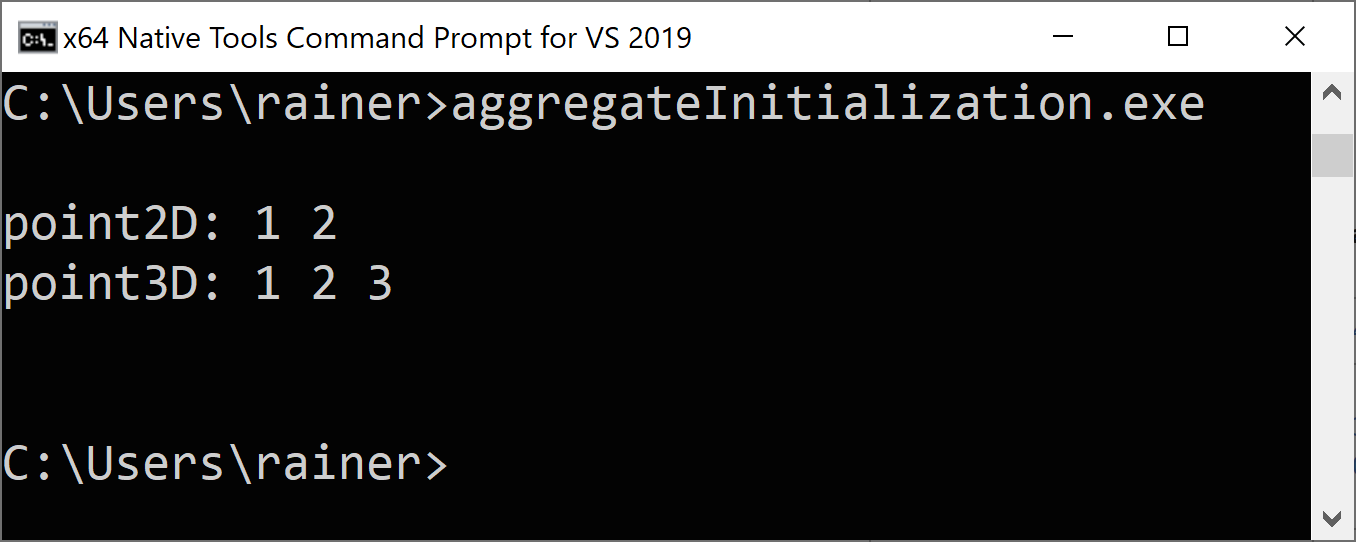
\includegraphics[width=0.8\textwidth]{content/3/chapter4/images/32.png}\\
Aggregate initialization
\end{center}

Based on aggregate initialization in C++11, we get designed initializers in C++20. At the end of 2020, only the Microsoft compiler supports designated initialization completely.

\subsubsubsection{4.4.2\hspace{0.2cm} Named Initialization of Class Members}

Designated initialization enables the direct initialization of members of a class type using their names. For a union, only one initializer can be provided. As for aggregate initialization, the sequence of initializers in the curly braces has to match the declaration order of the members.

\noindent
Designated initialization
\begin{lstlisting}[style=styleCXX]
// designatedInitializer.cpp

#include <iostream>

struct Point2D{
	int x;
	int y;
};

class Point3D{
public:
	int x;
	int y;
	int z;
};

int main(){
	
	std::cout << '\n';
	
	Point2D point2D{.x = 1, .y = 2};
	Point3D point3D{.x = 1, .y = 2, .z = 3};
	
	std::cout << "point2D: " << point2D.x << " " << point2D.y << '\n';
	std::cout << "point3D: " << point3D.x << " " << point3D.y << " "
							 << point3D.z << '\n';
	
	std::cout << '\n';
	
}
\end{lstlisting}

Lines 21 and 22 use designated initializers to initialize the aggregates. The initializers such as .x or .y are often called designators.

\begin{center}
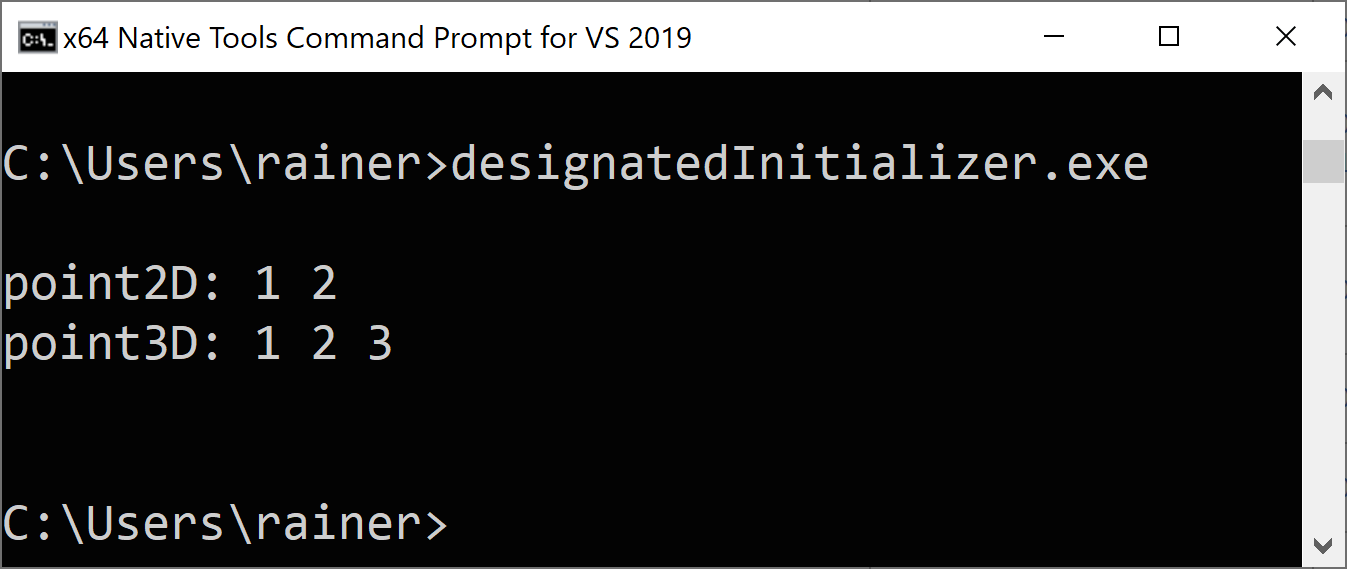
\includegraphics[width=0.8\textwidth]{content/3/chapter4/images/33.png}\\
Designated Initializers
\end{center}

The members of the aggregate can already have a default value. This default value is used when the initializer is missing. This does not hold for a union.

\noindent
Designated initializers with defaults
\begin{lstlisting}[style=styleCXX]
// designatedInitializersDefaults.cpp

#include <iostream>

class Point3D{
public:
	int x;
	int y = 1;
	int z = 2;
};

void needPoint(Point3D p) {
	std::cout << "p: " << p.x << " " << p.y << " " << p.z << '\n';
}

int main(){
	
	std::cout << '\n';
	
	Point3D point1{.x = 0, .y = 1, .z = 2}
	
	std::cout << "point1: " << point3D.x << " " << point3D.y << " "
							<< point3D.z << '\n';
							 
	Point3D point2;		 
	std::cout << "point2: " << point2.x << " " << point2.y << " "
							<< point2.z << '\n';
				
    Point3D point3{.x = 0, .z = 20};			 
	std::cout << "point3: " << point3.x << " " << point3.y << " "
							<< point3.z << '\n';
	
	// Point3D point4{.z = 20, .y = 1}; ERROR
	
	needPoint({.x = 0});
	
	std::cout << '\n';
	
}
\end{lstlisting}

Line 20 initializes all members, but line 24 does not provide a value for the member x. Consequently, x is not initialized. It is fine if you only initialize the members that don’t have a default value, such as in line 28 or line 34. The expression in line 32 would not compile because z and y are in the wrong order.

\begin{center}
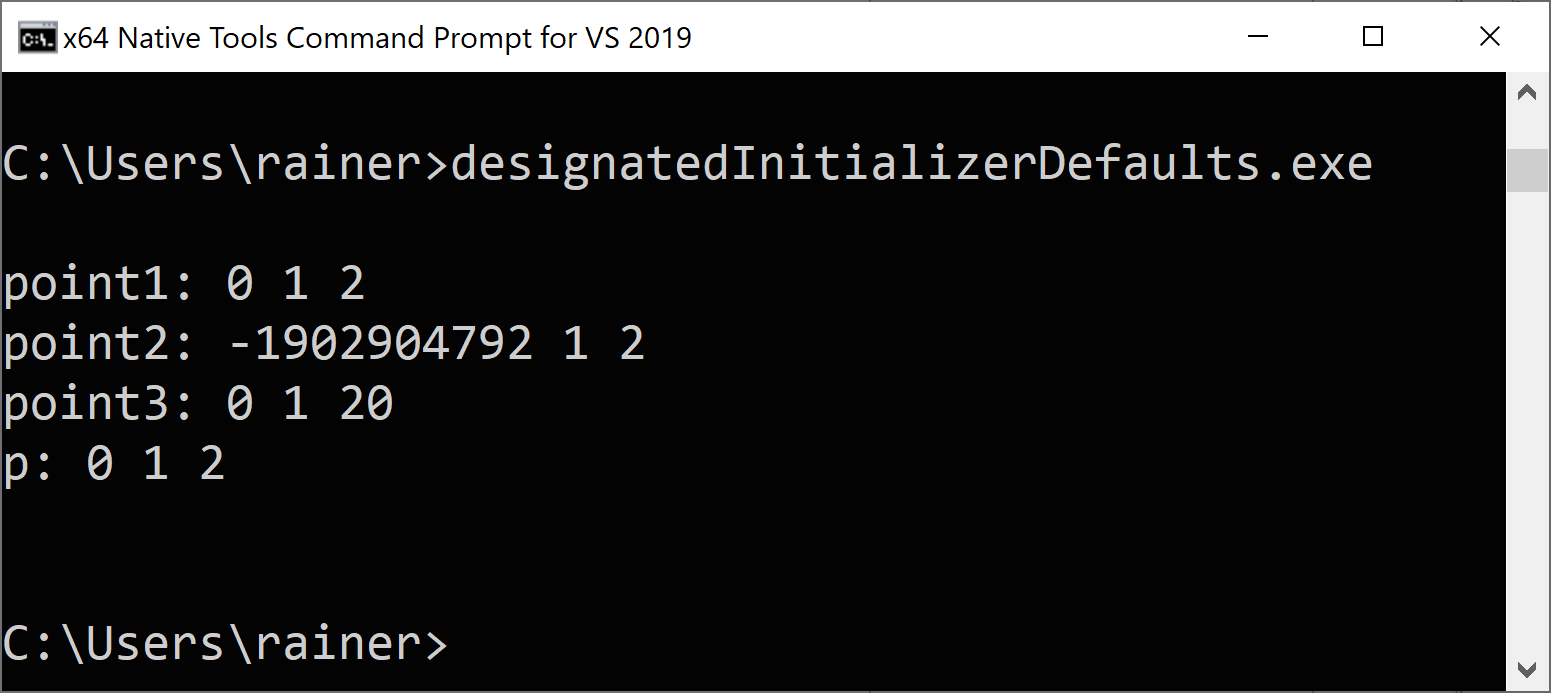
\includegraphics[width=0.8\textwidth]{content/3/chapter4/images/34.png}\\
Designated initializers with defaults
\end{center}

Designated initializers detect narrowing conversions. Narrowing conversion results in the loos of precision.

\noindent
Designated initializers detect narrowing conversion
\begin{lstlisting}[style=styleCXX]
// designatedInitializerNarrowingConversion.cpp

#include <iostream>

struct Point2D{
	int x;
	int y;
};

 class Point3D{
public:
	int x;
	int y;
	int z;
};

int main(){
	
	std::cout << '\n';
	
	Point2D point2D{.x = 1, .y = 2.5};
	Point3D point3D{.x = 1, .y = 2, .z = 3.5f};
	
	std::cout << "point2D: " << point2D.x << " " << point2D.y << '\n';
	std::cout << "point3D: " << point3D.x << " " << point3D.y << " "
							 << point3D.z << '\n';
	
	std::cout << '\n';

}
\end{lstlisting}

Line 21 and line 22 produce compile-time errors, because the initialization .y = 2.5 and .z = 3.5f would cause narrowing conversion to int.

\begin{center}
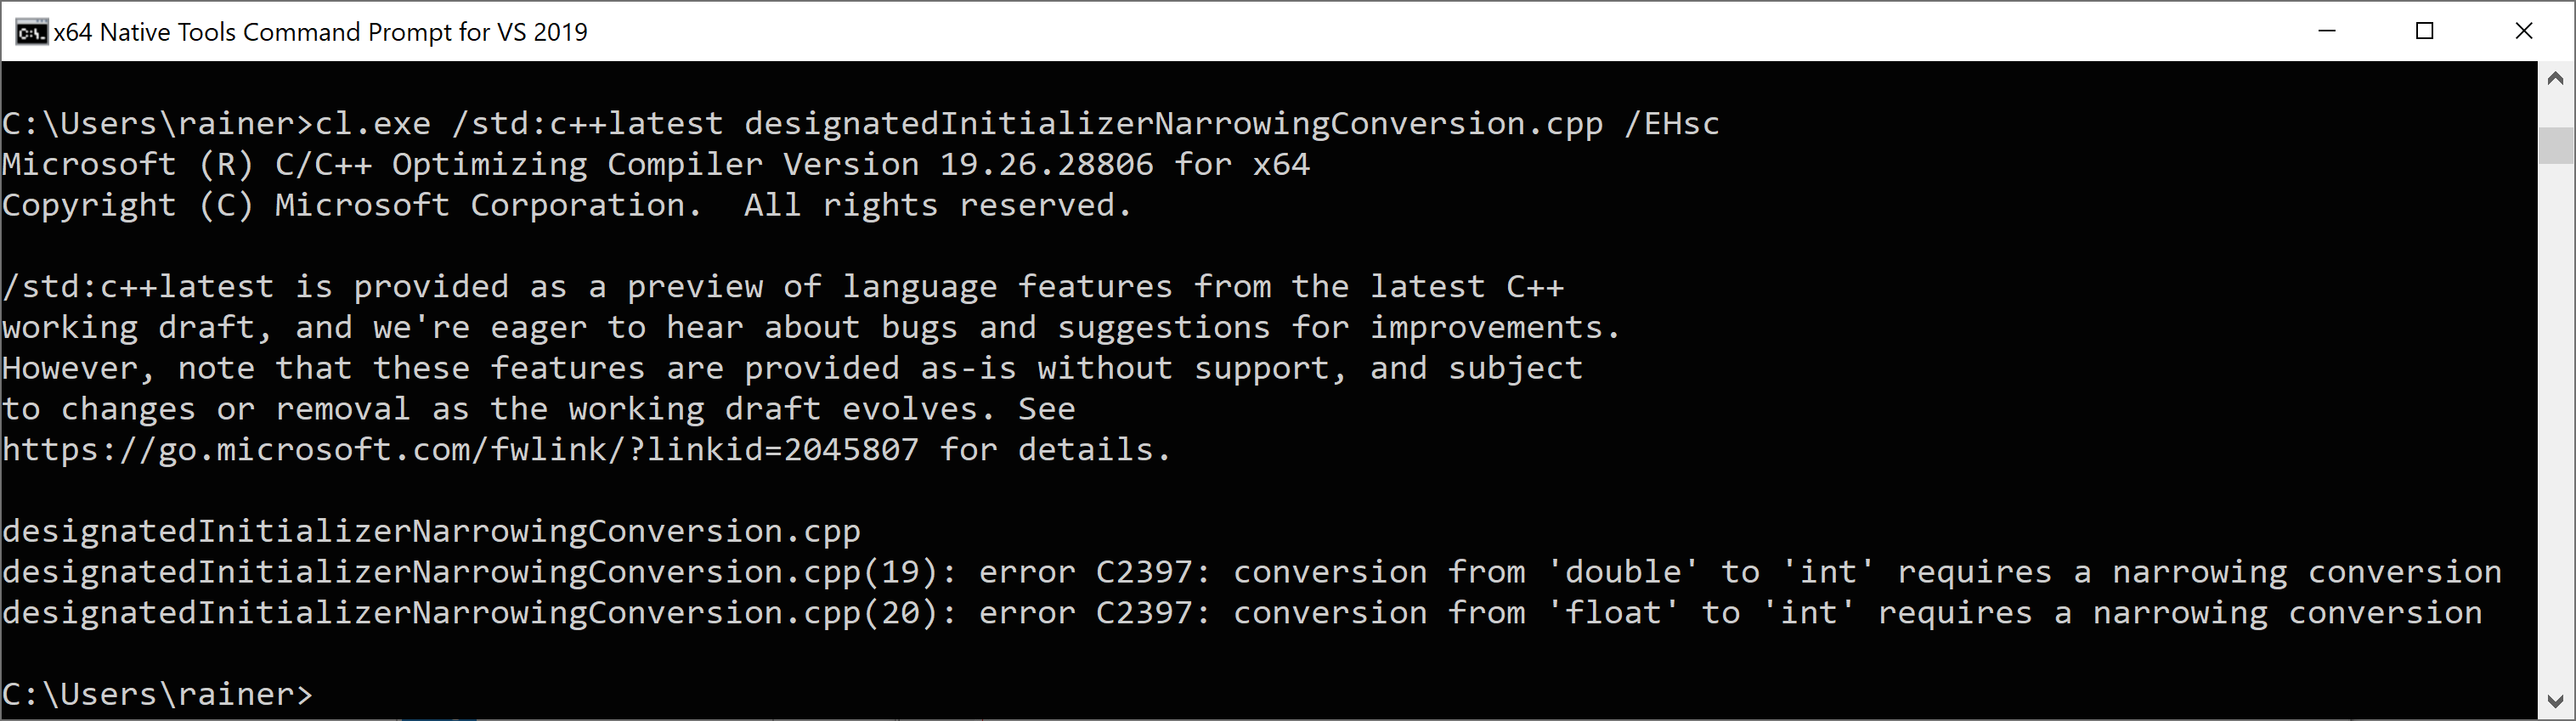
\includegraphics[width=0.8\textwidth]{content/3/chapter4/images/35.png}\\
Designated initializers detect narrowing conversion
\end{center}

Interestingly, designated initializers in C behave differently from designated initializers in C++.

\begin{tcolorbox}[colback=red!5!white,colframe=red!75!black,title={Similarity to Python}]
C designated initializers support use cases that are not supported in C++. C allows

\begin{itemize}
\item 
initializing the members of the aggregate out-of-order

\item 
initializing the members of a nested aggregate

\item 
mixing designated initializers and regular initializers

\item 
designated initialization of arrays
\end{itemize}

The proposal \href{http://www.open-std.org/jtc1/sc22/wg21/docs/papers/2017/p0329r4.pdf}{P0329R4} provides self-explanatory examples for these use cases:

\noindent
Difference between C and C++
\begin{lstlisting}[style=styleCXX]
struct A { int x, y; };
struct B { struct A a; };
struct A a = {.y = 1, .x = 2}; // valid C, invalid C++ (out of order)
int arr[3] = {[1] = 5}; // valid C, invalid C++ (array)
struct B b = {.a.x = 0}; // valid C, invalid C++ (nested)
struct A a = {.x = 1, 2}; // valid C, invalid C++ (mixed)
\end{lstlisting}

The rationale for this difference between C and C++ is also part of the proposal: “In C++, members are destroyed in reverse construction order and the elements of an initializer list are evaluated in lexical order, so field initializers must be specified in order. Array designators conflict with lambda-expression syntax. Nested designators are seldom used.” The paper continues to argue that only out-of-order initialization of an aggregate is commonly used.

\end{tcolorbox}	

\begin{tcolorbox}[colback=blue!5!white,colframe=blue!75!black,title={Distilled Information}]
Designated initialization is a special case of aggregate initialization and enables it to initialize the class members using their name. The initialization order must match the declaration order.
\end{tcolorbox}	






